\documentclass{article}
\usepackage{natbib}
\usepackage{graphicx}
\usepackage{float}
\usepackage{listings}
\usepackage{url}

\title{High-Performance Data Analysis on JANUS using Apache Spark}
\author{Nick Vanderweit \\
        Ning Gao \\
        Anitha Ganesha \\
        Michael Kasper}

\begin{document}
\maketitle

\section{Introduction}
Over the past decade, there has been considerable interest in high-level
strategies for evaluating algorithms in parallel over large data sets.
Google's seminal MapReduce paper \citep{dean-mapreduce} describes such a
general strategy, which had already been in use at Google at the time of
publication, for building highly-scalable parallel applications out of small
serial functions. In general, phrasing data parallelism in terms of
higher-order functions on parallel data structures has proven fruitful
for many applications. In this paper, we evaluate Spark, a library
designed to address some of the shortcomings of MapReduce, on an existing
supercomputer.

In the MapReduce model, data is broken into \emph{splits} of a given size
before processing. These are stored on a distributed filesystem as key/value
pairs. The master node then distributes splits among the remaining workers.
Each of these workers runs a \emph{Map} on its split, computing for each
key/value pair $(k_1, v_1)$ another pair $(k_2, v_2)$. Each of these output
pairs is stored on the filesystem and the master is informed of their
locations. The master node proceeds by forwarding these intermediate pairs to the
\emph{Reduce} workers, which are responsible for combining the results for each
intermediate key.

A commonly-used example for this process is a distributed word count. First,
the input file (e.g. a large database dump containing posts on an Internet
forum) is broken into splits of a given size (say 64MB). The splits store
$(k, v)$ pairs such that each $v$ is a record (a post). The \emph{Map} task
is responsible for mapping each record to a set of $(\mbox{word}, \mbox{count})$
pairs, which are written to the filesystem.

The next step is for a \emph{Reduce} worker to sort these records by key
and then sum together the values for each given key, and write out
a set of (word, count) records where the keys are now unique.

This simple example has interesting implications for MapReduce in general.
We can see that \emph{Map} tasks are highly-parallel, but \emph{Reduce}
introduces a serial bottleneck. In cases like parallel word count, where the
\emph{Reduce} is associative and commutative (i.e. forms a commutative
semigroup over the set of values), there is an additional opportunity for
parallelism. As such, MapReduce provides an additional task, called a
\emph{Combiner}, which assumes this structure and can be used to distill
the intermediate $(k, v)$ pairs before a \emph{Reduce}.

We can also see from this example a significant limitation of MapReduce: each
intermediate $(k, v)$ set is written to the distributed filesystem.  As such,
in order for MapReduce to be efficient, the individual tasks must be very
large.

However, some algorithms are not well-described by a simple map-and-then-reduce
pattern, and require multiple iterations.  If each iteration is small, the
algorithm's performance will be bottlenecked by this file I/O. For these
problems, another approach is needed.

Spark was designed at the UC Berkeley AMPLab to address these concerns using a
more flexible abstraction for distributed data \citep{zaharia}. Rather than
assuming that all intermediate data is stored on a filesystem, Spark uses
\emph{Resilient Distributed Datasets}, or RDDs, to represent data that is
stored on disk, cached in memory, or possibly has not been computed yet at all
\citep{zaharia_rdd}.  It is primarily targeted toward Scala, a statically-typed
functional language for the Java Virtual Machine.

\section{Overview}
One of the key insights of Spark is that reducing the strictness of a
computation can offer large gains in performance. This lies at the heart
of the notion of RDDs: it is often more efficient to represent a \emph{recipe}
for a result than to represent the result itself, especially when the data sets
are arbitrarily large. Some programmers may be familiar with the related
notion of a \emph{thunk} in functional programming.

To demonstrate this idea, consider the following code snippet in a
functional language like ML:

\begin{lstlisting}[language=ML]
let rdd = ...
let mapped = map (fun x -> x * 2) rdd
let filtered = filter (fun x -> x mod 4 == 2) mapped
let sum = List.fold_left (fun x y -> x + y) 0 filtered
...
\end{lstlisting}

In the MapReduce model, there would be a strict filesystem write after each of
these lines.  Spark does not impose such a restriction, and allows the data to
persist in memory between operations. In fact, it even goes a step beyond this.
By default, RDDs are stored lazily as chains of computations that would
produce an output value. This has several advantages: for one, it is much
more practical to recover failed nodes with such a recipe in hand. Also,
storing computations as a lazy data structure permits certain optimizations.
For instance, the above example contains a \texttt{map} composed with a
\texttt{filter}. If this computation is expressed as a data structure,
the Spark environment can dynamically optimize it to:

\begin{lstlisting}[language=ML]
let rdd = ...
let filtered = filter (fun x -> (x * 2) mod 4 == 2) mapped
let sum = List.fold_left (fun x y -> x + y) 0 filtered
...
\end{lstlisting}

This kind of optimization is known as \emph{deforestation}, the elimination
of intermediate data structures, and is used to greatly improve data
locality \citep{wadler}.

In general, this way of identifying data with its lineage is a very powerful
way to perform \emph{batch computations} on data, which means applying the same
transformation over many elements of a distributed data structure. Like
MapReduce, Spark is not well-suited for applications where each parallel
tasks requires communication with other threads.

Spark provides APIs for Java, Python, and Scala, although the Scala API seems
to be the most common. This is likely because of Spark's heavy use of
higher-order functions on data structures, which is a staple of
functional programming.

\emph{Bagel} is an implementation of the Google Pregel graph processing framework
for Spark, which works on a distributed set of $(k, v)$ pairs, where $k$ is
a vertex ID and $v$ is a vertex with its state. This allows algorithms like
PageRank to be written simply, and we use this to evaluate Spark's performance
on iterative algorithms.

Spark also has a Hive-compatible query system called Shark. Though it is beyond
the scope of this project, Shark allows efficient interactive data querying
using an SQL-like syntax.

\section{Evaluation}
We conducted our evaluation of the Spark system on the University of
Colorado's JANUS supercomputer. JANUS consists of 1,368 nodes, each containing
two six core Intel Xeon Westmere-EP chips at 2.8 GHz, for a total of 12 cores
per node. Additionally, each core has 2 GB of 1333 MHz DDR RAM, for a total of
24 GB per node \citep{tufo}. In our research, we employed Spark version
0.8.0 along with Scala version 2.9.3. During our testing of the Spark system,
we access input files from JANUS' lustre distributed file system. Our aim was
to assess the Spark runs on JANUS and determine optimal configurations to
achieve the best performance.

\subsection{Testing}
Following the example from Google's first paper on MapReduce, the first test we
performed was a parallel grep \citep{dean-mapreduce}. Here an application would
scan through a large test file, looking for lines that matched a given regular
expression, finally returning the total number of matched lines. Two series of
tests were run on two different files sizes. During these tests, we wanted to
see how Spark scales in an ideal setting, where the entire data set fit in
memory. This way we avoid the large performance hit Spark takes writing
intermediate results to disk. Given that each node has a total of 24 GB of RAM,
we limited our first problem size to 20GB. This allowed a single node to
contain the entire problem in memory, leaving sufficient memory space for the
OS and other supporting processes. We executed this first test with 1 to 5
nodes. The second test we performed was run with 5 to 50 nodes, each processing
a 100GB file.

Ten trials were performed for each test, allows us to compute average
runtimes. To compute the speedup, Spark runtimes were compared to the UNIX grep
command's serial runtime on the same file. Finally, during our first test on the
20 GB file, we evaluated performance using a different number of workers per
node. In Spark, a worker is an executor with its own JVM which processes its
own portion of the distributed data set. By default, a single worker is
employed on each node. For this test, we wanted to see if this was the ideal
setting for running Spark on JANUS.

% page rank
    % overview
    % ...

\subsubsection{PageRank}   
Since Spark system is an in-memory cluster computing system, the power of such a system should be exploited by applications that runs several iterations on the same data. 

As an example of iterative algorithms the \emph{Page Rank} algorithm was chosen.
The original pagerank algorithm was developed by Google websearch engine which enabled them to rank the webpages in their search engine.

\emph{Data set}:
The source of the dataset is DBPedia, a crowd sourced community that extracts structured information from wikipedia and makes it available on the web. \citep{[??]} There are different formats of wikipedia datasets available online. For our experiments we chose the wikipedia pagelink dataset \citep{[??]} , this contains
internal links between the DBPedia instances extracted from the internal links of the wikipedia articles making it apt for the any datamining related analysis including Pagerank algorithm. Therefore this dataset was chosen for the experiment.
The overall size of this dataset is 25GB.
The format of the data is \{ source url \} \{ some configuration \} \{ dest url \}
For the pagerank algorithm, only the source url and the dest url is needed.Therefore the dataset was was preprocessed to filter out the only the necessary information.

If the entire dataset is assumed to be represented by a huge graph, then here each DBPedia instance maps to a wikipedia article or a page which inturn could be mapped to a vertex of the graph. And the links between the instances could be mapped to  
edges of the graph.


\begin{figure}
\centering
  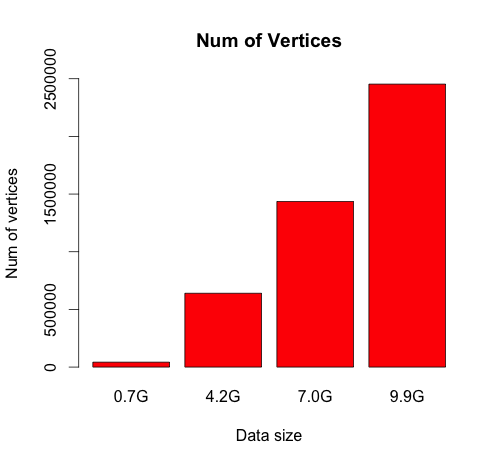
\includegraphics[width=80mm]{images/numVertices.png}
  \caption{The vertices count over various dataset size}
  \label{fig:numvertices}
\end{figure}

\begin{figure} 
  \centering
  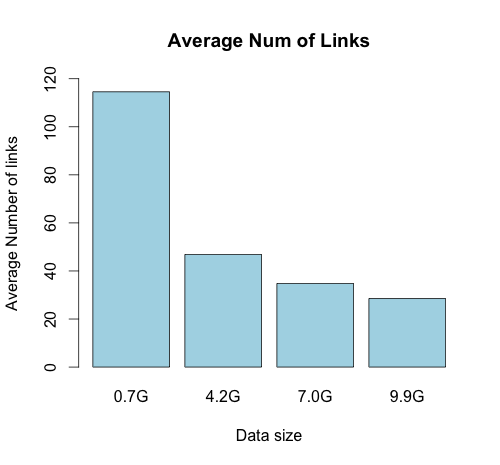
\includegraphics[width=80mm]{images/numLinks.png}
  \caption{The average edge count per vertex for various dataset size}
  \label{fig:numlinks}
\end{figure}

The figure \ref{fig:numvertices} shows the variation in the no of vertices count for different dataset size which from ~40,000 nodes and the figure \ref{fig:numlinks} shows  the average number of links or edges per vertex for a smaller dataset is much higher as compared to the larger dataset. The smaller dataset are the first few DBPedia instances of the larger dataset. The first few pages probably have more links compared the pages in the end of the dataset and hence the average is linearly decreasing.


\emph{Algorithm:}
The basic idea of the page rank algorithm is to assign scores to the pages based on the following two aspects of the page.
	\begin{enumerate}
		\item {\centering pages with higher incoming links get high rank.}
		 \item {\centering pages with links from a high rank page also gets high rank.}
	\end{enumerate}

The pseudocode of the algorithm is as follows:
\begin{enumerate}
	\item {\centering Assign every page a rank of 1.}
	\item {\centering On each iteration have page p contribute to rankp/ |neighbours|p to its neighbors.}
	\item {\centering Set each page ranks to \(0.15 + 0.85  *  contributions\)}.
	\end{enumerate}   
	
The scala implementation of this algorithm is as shown below:
\begin{lstlisting}[language=ML]
vallinks =// RDD of (url, neighbors) pairs
varranks =// RDD of (url, rank) pairs
for(i<- 1 to ITERATIONS) 
{
  valcontribs=links.join(ranks).flatMap{
  case (url, (links, rank)) => links.
  map( dest=> (dest, rank/links.size))
  }
  ranks =contribs.reduceByKey(_ + _).
  mapValues(0.15 + 0.85 * _)
}
ranks.saveAsTextFile(...) 
\end{lstlisting}	
     
\emph{Bagel}:
The Bagel programming model was developed by spark.This is the implementation of the graph processing framework developed by google called the \emph{Pregel} system[??]. Bagel is still in the development stage where in more features are being added to the basic graph computation framework.

Any graph algorithm runs for several iterations and each iteration is called a Superstep.The graph is represented as a distributed dataset of $(K,V)$ pairs.  Here, the keys are vertex IDs, the values are vertex and associated states of the vertices.Every vertex in the graph will be associated with a user specified function.In each superstep, the algorithm runs the function associated with the vertex using the messages recieved from the previous superstep. The output is a new vertex state and a list of all outgoing messages which is then sent to all the other dependent vertices which is then used as input for the next iteration.

For the pagerank algorithm, as previously explained the vertices are pages and the edges are links.The list of messages generated at every iteration is the contribution of the pagerank for all its outgoing links.

Bagel provides APIs for vertices, edges and messages which could be extended to customize for any algorithm.This enables the user to write any compilcated code within few lines of code.

Further, bagel also provides combiner utility where in a reduction operation is applied on the outgoing message which reduces the communication overhead.The aggregator utility helps in reducing the message across all nodes for all vertices of the graph after every superstep.

\emph{Hash Partitioner}:The algorithm makes use of a hash partitioner which is a Controlled data partitioning utility that reduces communication cost.Also, it keeps the information of how data was partitioned across jobs for further reduction of communication cost.

\emph{Kyro serialization}: For the bagel program a special form of serialization technique was used, this  serializes the object sent over the network that will be cached in serialized form. The kryo serialization is much faster than the default java serialization used in the spark system as it the communication cost.

\subsection{Results}
In the first grep test, we examined how Spark scales over a 20GB file using 1
to 5 nodes. Additionally, each trial was executed with a different number
workers per node. Figure \ref{fig:workNodeTime} shows the average runtimes as
the number of nodes increases. Each line in this graph represents a different
number of workers per node. We clearly can see from this graph that 6 and 12
workers per node yields significantly worse performance, while the results
produced by 1 to 3 workers is relatively equal.

    \begin{figure}[H]
        \centering
        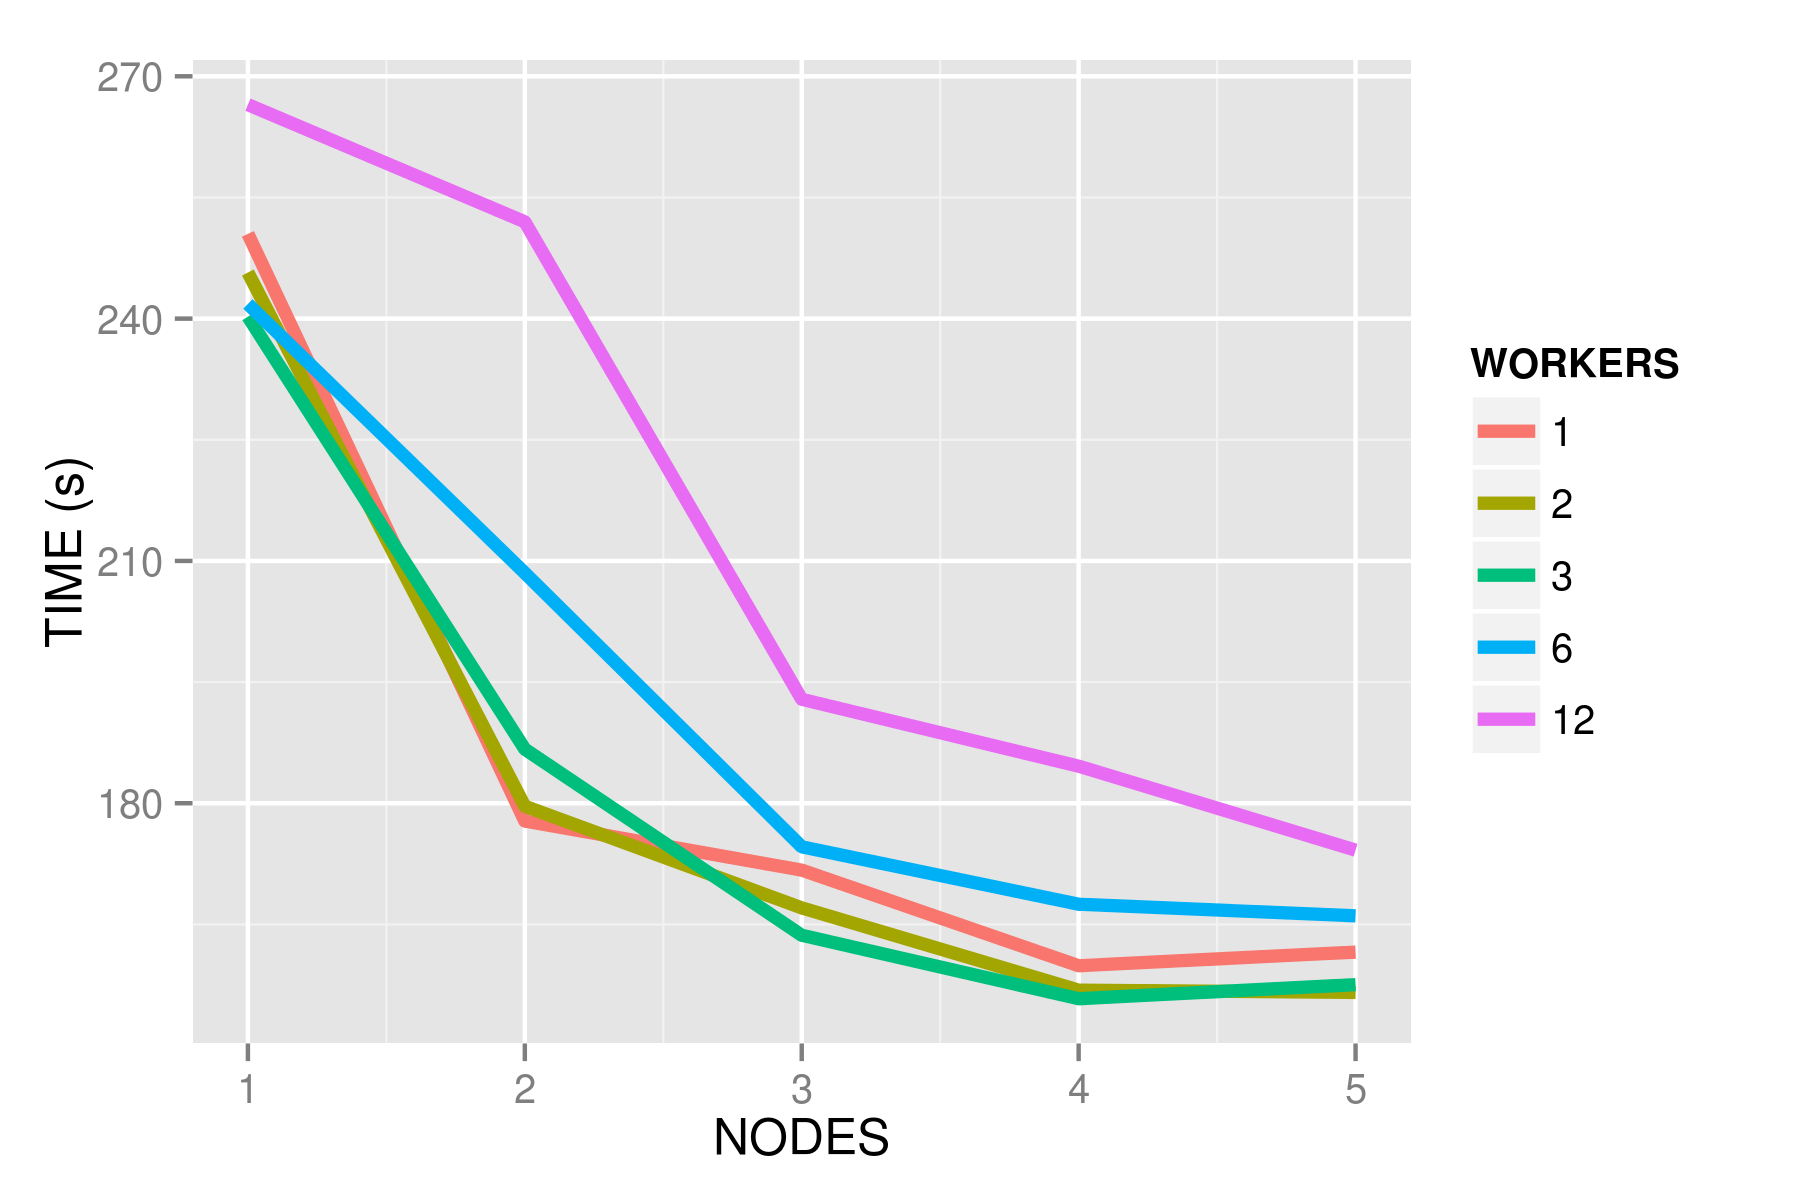
\includegraphics[width=90mm]{images/workerPerNodeTimes.png}
        \caption{Grep runtimes with different workers per node over 20GB file}
        \label{fig:workNodeTime}
    \end{figure}

Figure \ref{fig:workNodeSpeed} illustrates the results in terms of speedup.
Here we are comparing the resulting runtimes to the UNIX grep serial runtime of
1,120 seconds, processing the same 20 GB file. Note that here 1 node represents
12 cores. So the initial speedup between 3 and 4 is not as impressive as one
might expect. We also see that the speedup begins to level out around 4 nodes,
and in the case of 1 to 3 workers per node, it even decreases from 4 to 5
nodes.

    \begin{figure}[H]
        \centering
        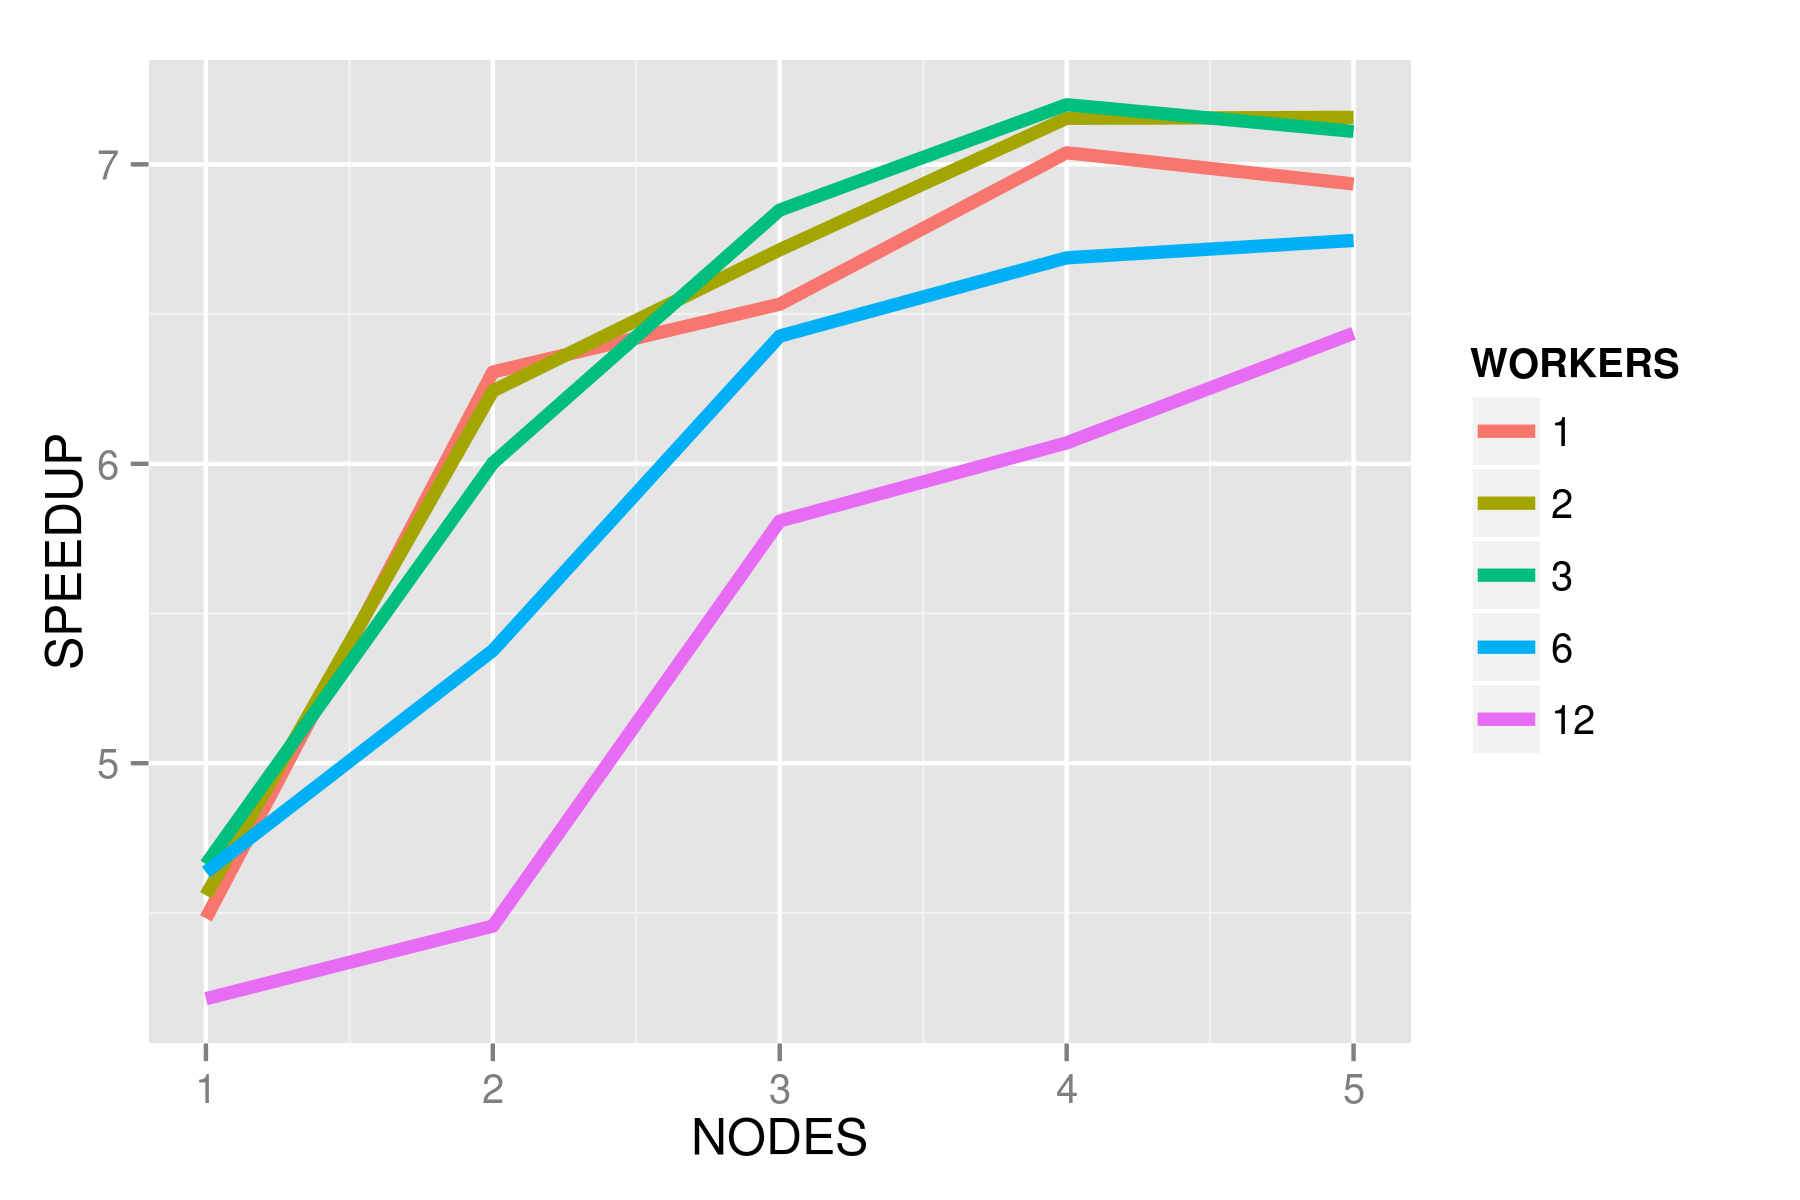
\includegraphics[width=90mm]{images/workerPerNodeSpeedup.png}
        \caption{Grep speedup with different workers per node over 20GB file}
        \label{fig:workNodeSpeed}
    \end{figure}

In the efficiency graph show in Figure \ref{fig:workNodeEff} we can see just
how well the cores are being utilized. As expected from the results shown in
the previous figures, the efficiency is quite poor. Employing a single node
starts just under 40\% efficiency. By the time we scale the problem to 5 nodes
(60 cores) we are just above 10\% efficiency.

    \begin{figure}[H]
        \centering
        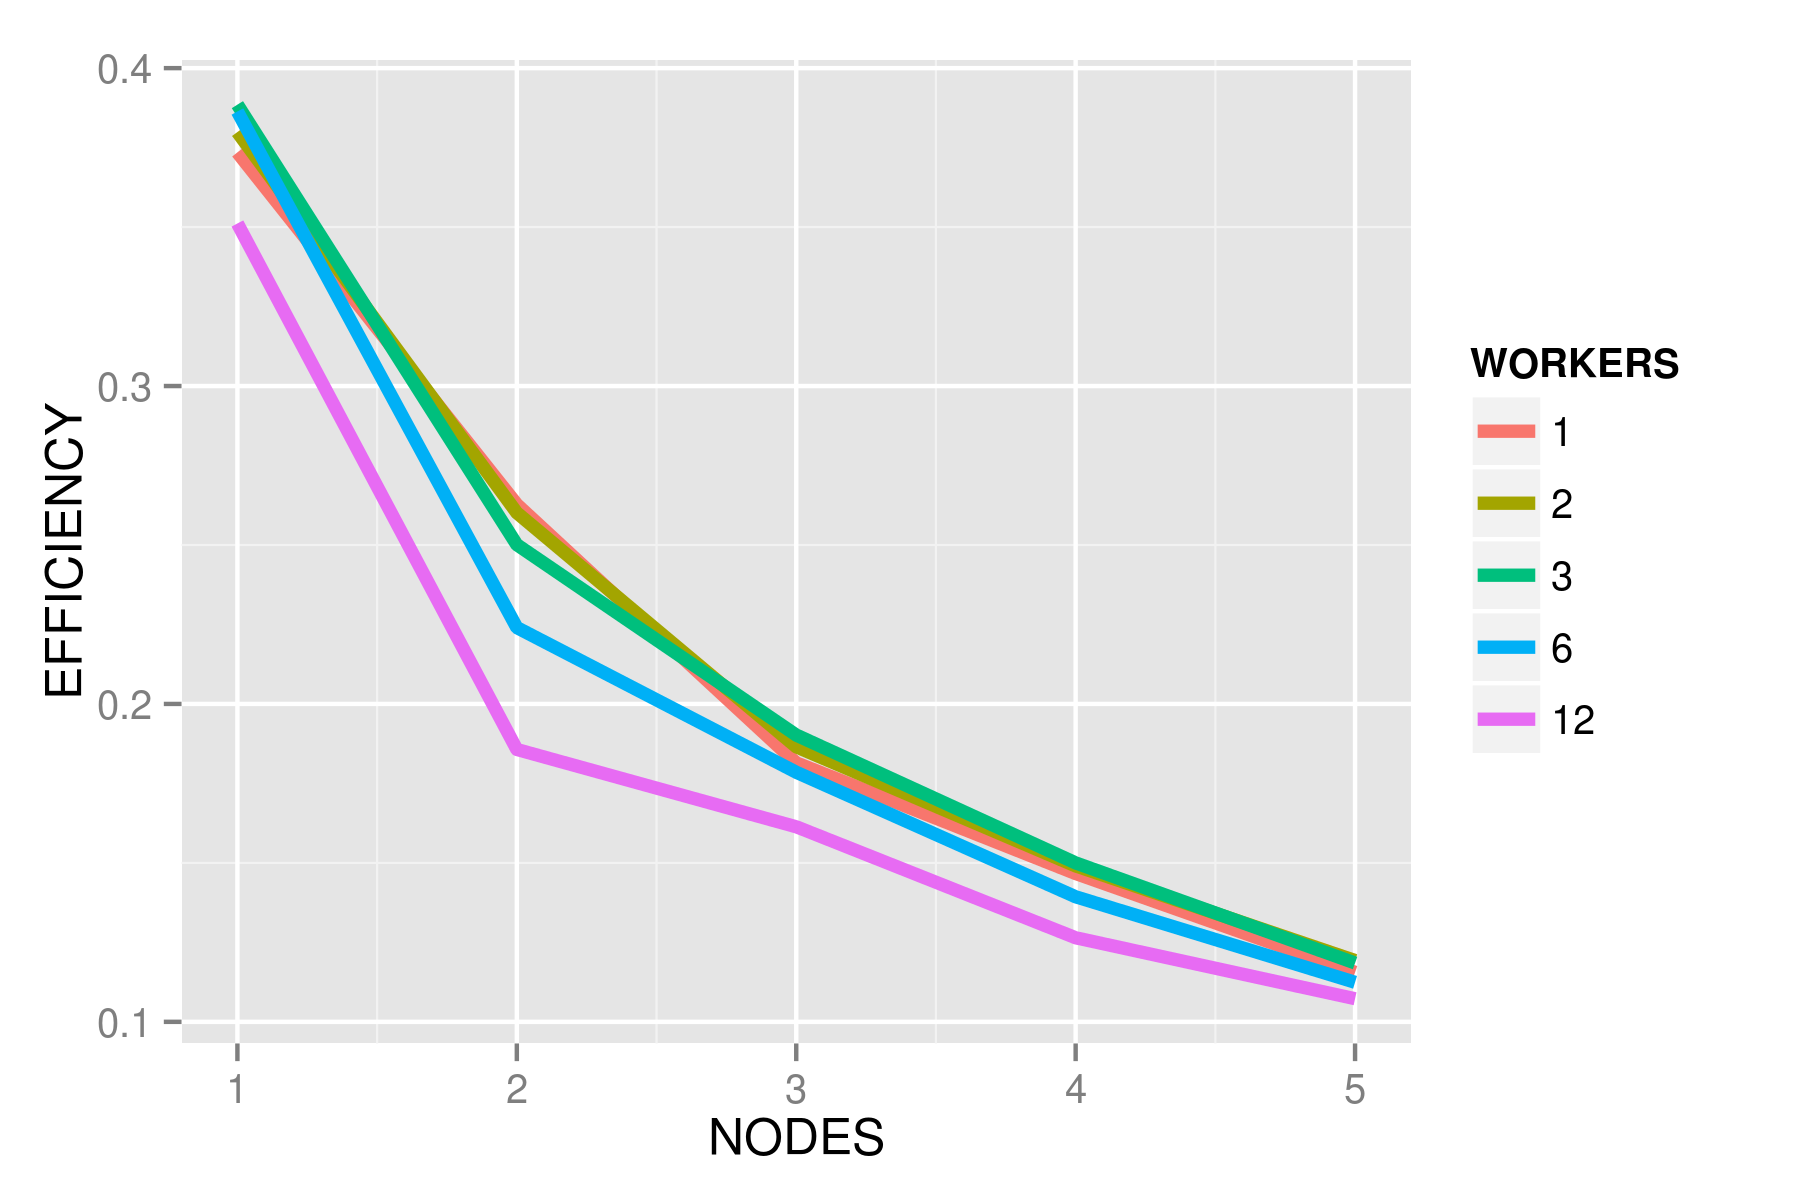
\includegraphics[width=90mm]{images/workerPerNodeEfficiency.png}
        \caption{Grep efficiency with different workers per node over 20GB file}
        \label{fig:workNodeEff}
    \end{figure}

Finally, Figure \ref{fig:workNodeKF} reflects the Karp-Flatt metric for the
runtime results. With the exception of the test using 12 workers per node (pink
line), we we see that the Karp-Flatt metric remains relatively constant, with
values between 0.12 and 0.14. This constant value would suggest that the
large serial portion of the application is what is preventing use from seeing
better scaling.

    \begin{figure}[H]
        \centering
        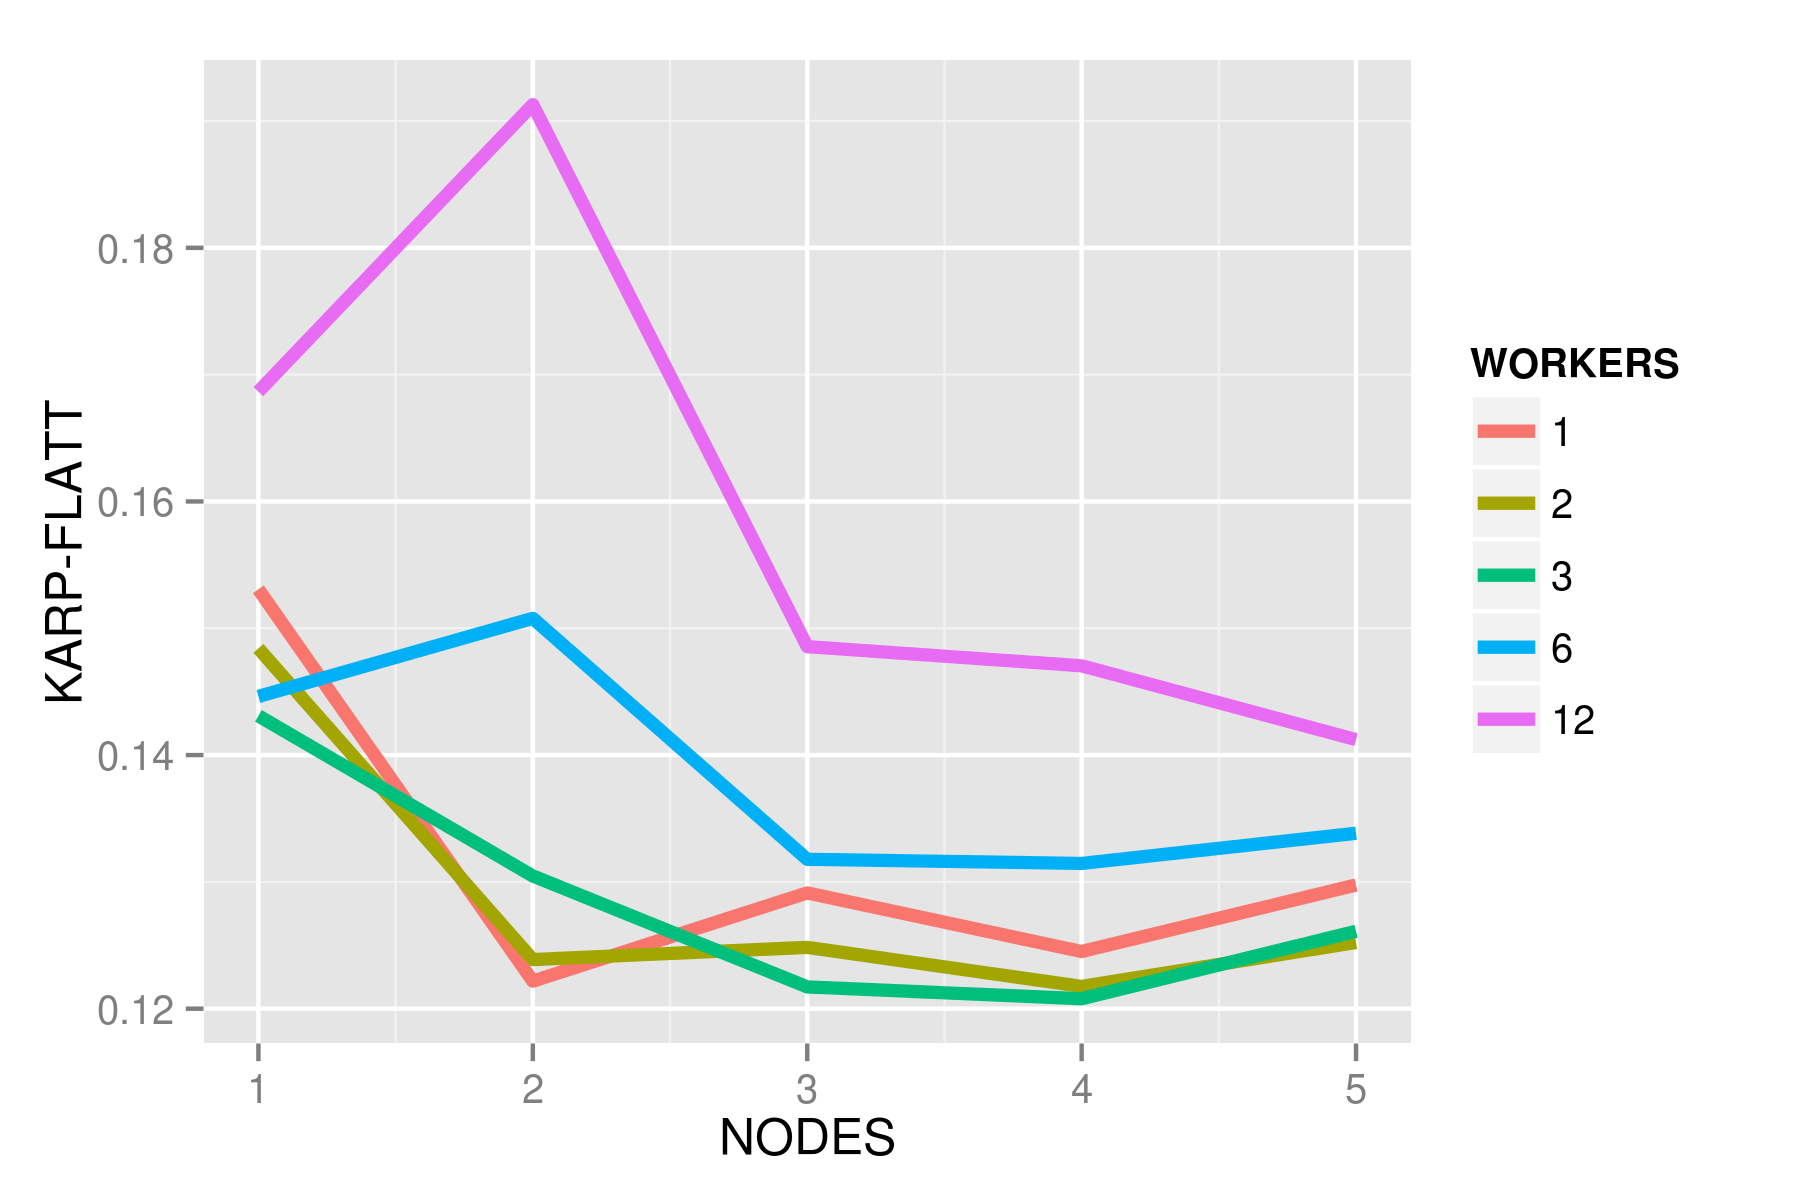
\includegraphics[width=90mm]{images/workerPerNodeKarpFlatt.png}
        \caption{Grep Karp-Flatt with different workers per node over 20GB file}
        \label{fig:workNodeKF}
    \end{figure}

To see if we could observe better scaling, we ran the same grep test over a
100 GB file. During this test, we also increased the number of nodes used,
starting with 5 and going to 50 nodes. Figure \ref{fig:bigTime} shows the
runtimes observed over this large problem.  Clearly there appears to be no
change in runtimes, as the runtimes hover around 500 seconds, regardless of the
number of nodes used.

    \begin{figure}[H]
        \centering
        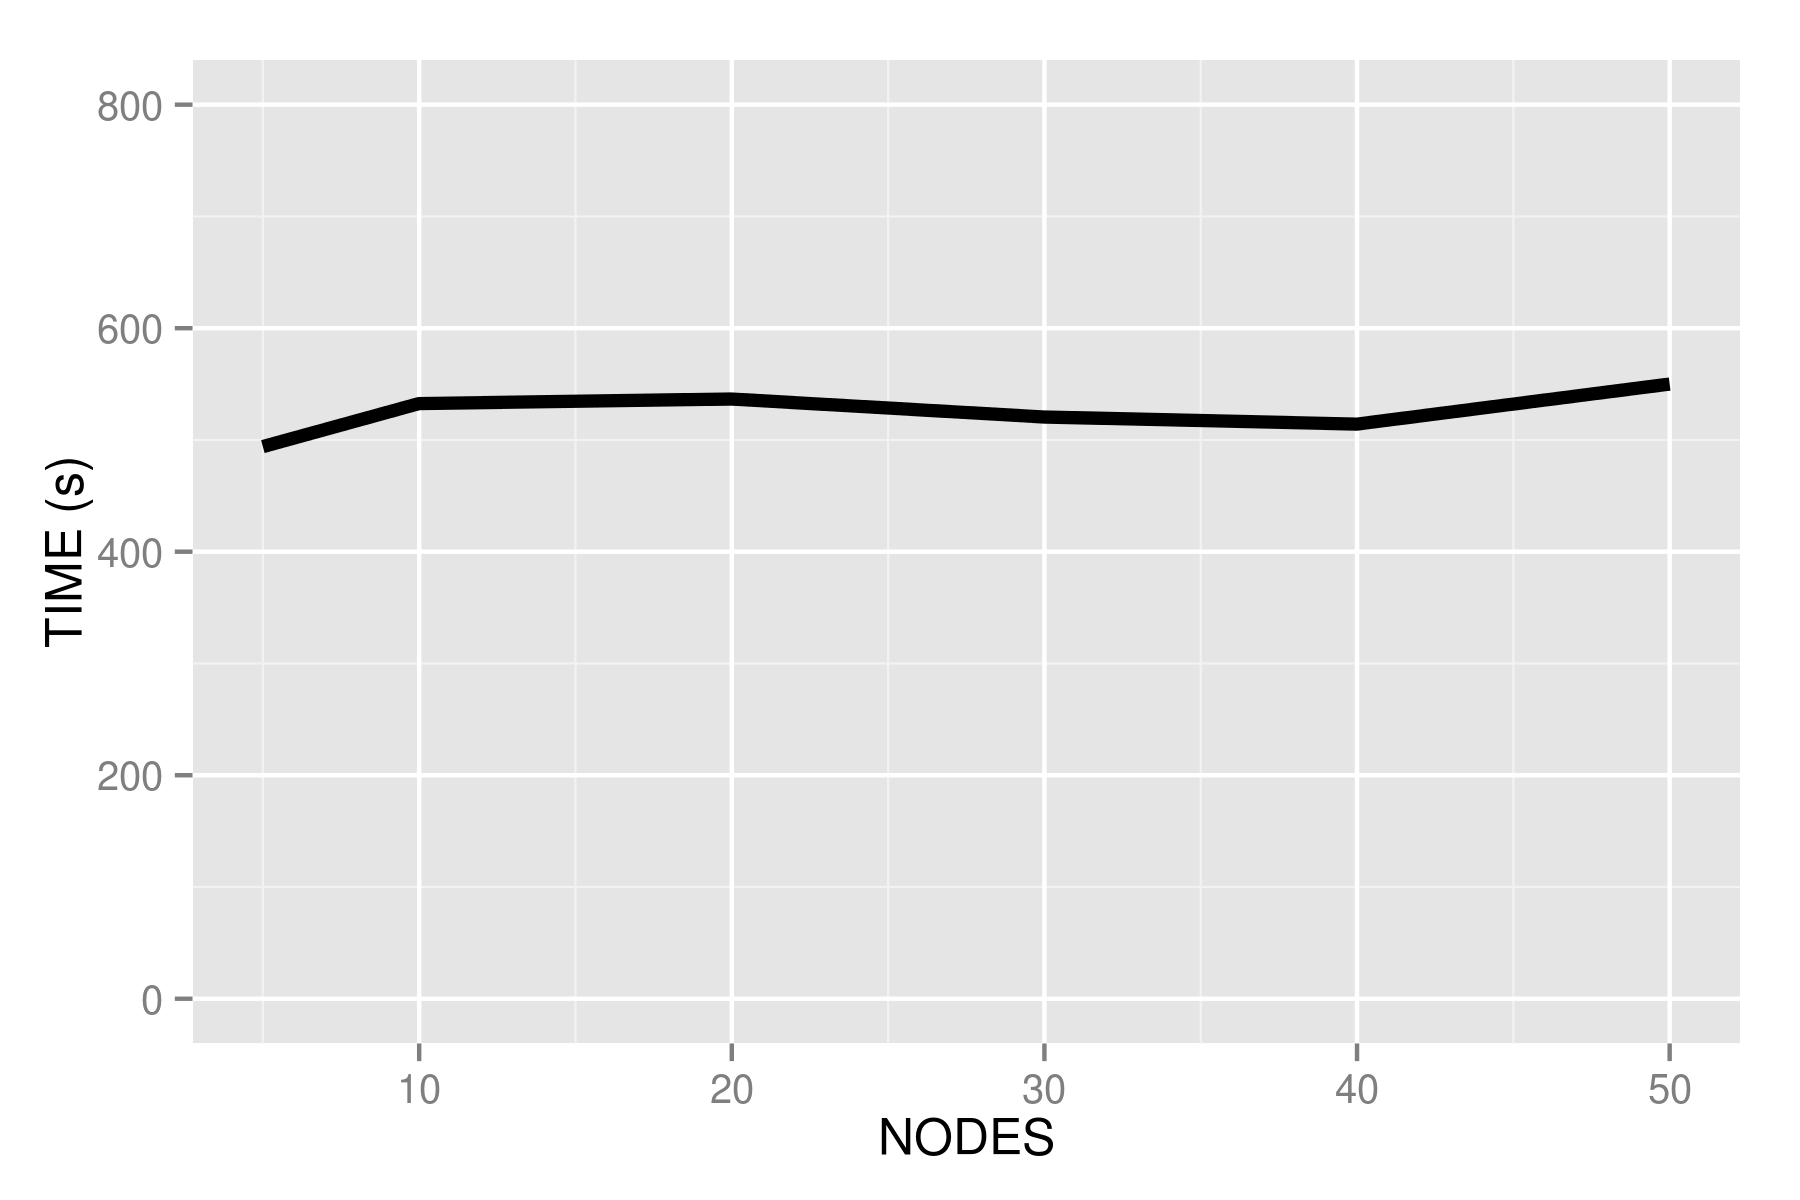
\includegraphics[width=90mm]{images/bigDataTimes.png}
        \caption{Average grep runtimes over 100GB file}
        \label{fig:bigTime}
    \end{figure}

Suspecting the short computational time of the grep search was negligible as
compared to the file load time, we began running our tests on the more
computationally expensive PageRank algorithm. We ran five tests in total,
measuring the amount of wall clock time each took to compute.

    \begin{figure}[H]
        \centering
        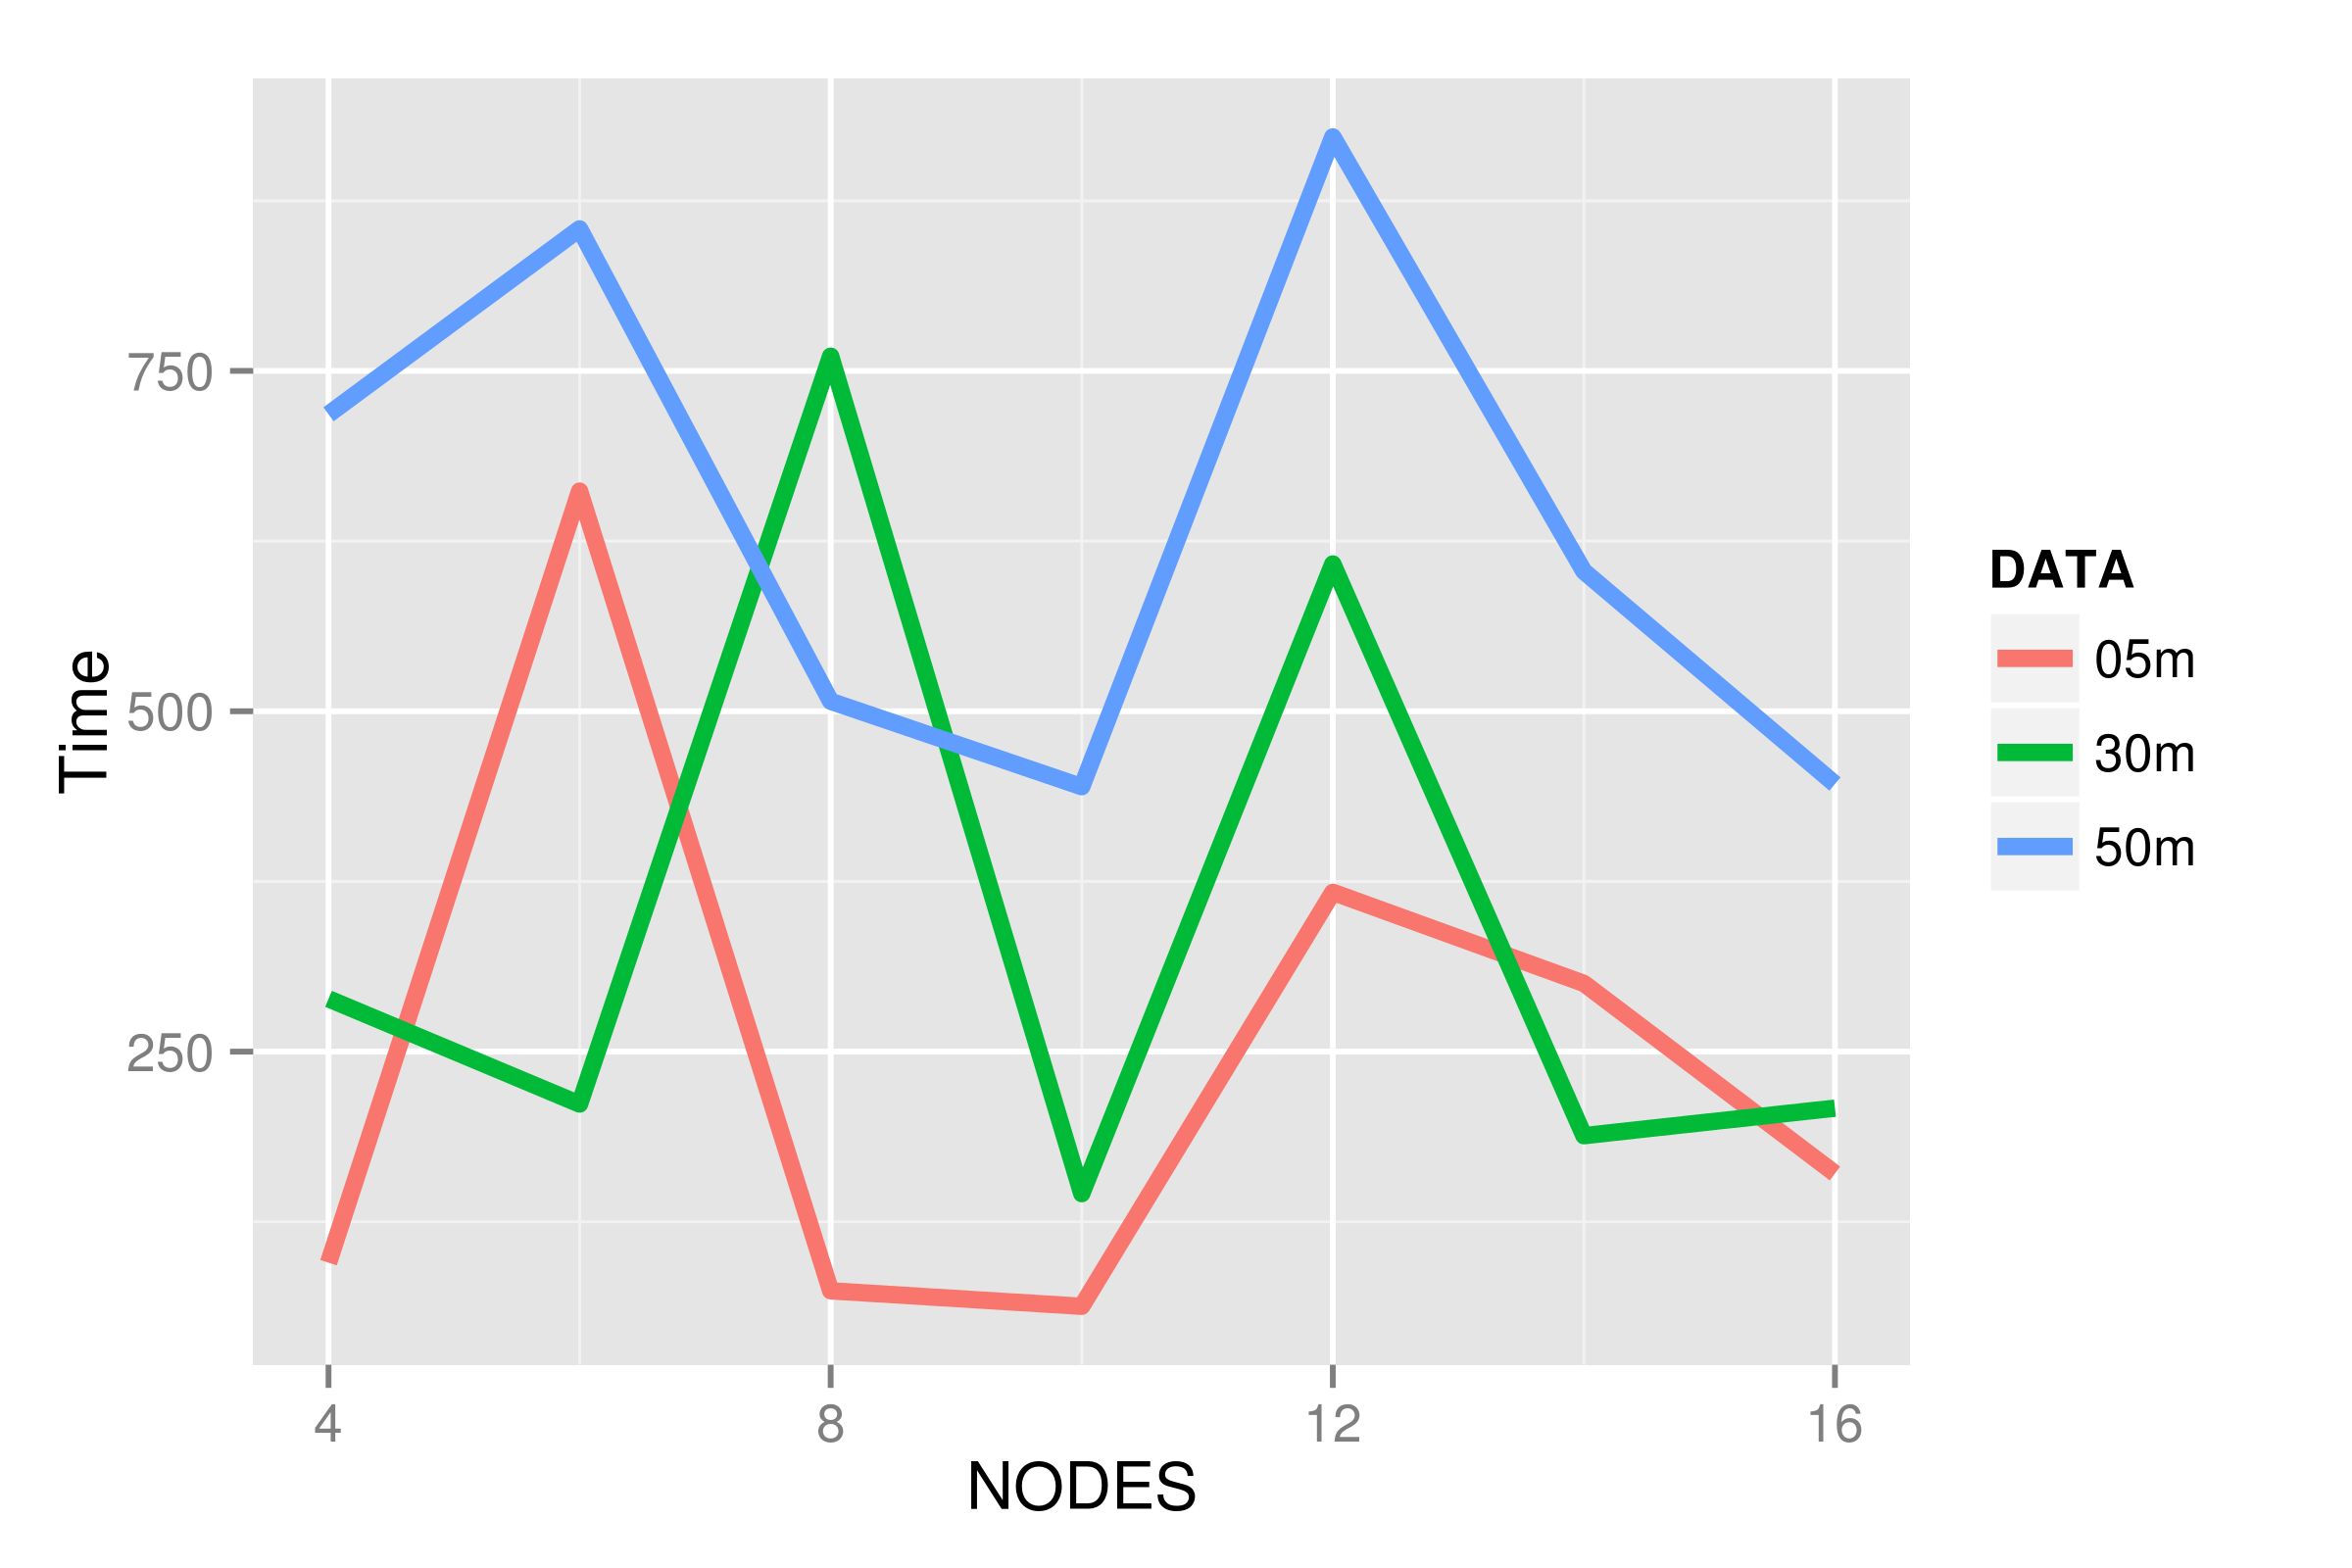
\includegraphics[width=90mm]{images/scalability.png}
        \caption{Scalability Test for Pagerank}
        \label{fig:scalability}
    \end{figure}


We tested a Bagel implementation of PageRank on several of 5 million links, 30
million links, and 50 million links. We ran these computations on allocations
ranging from 4 to 16 nodes, incrementing by two.  As shown in Figure
\ref{fig:scalability}, for the scalability test, the larger the dataset is, the
better the scalability is because the ratio of computation to communication is
large. We had to run on a small dataset because of a technical problem with our
Spark installation.\footnote{
\url{https://groups.google.com/forum/#!topic/spark-users/-nsoF7oonOM}}

\begin{figure}[H]
        \centering
        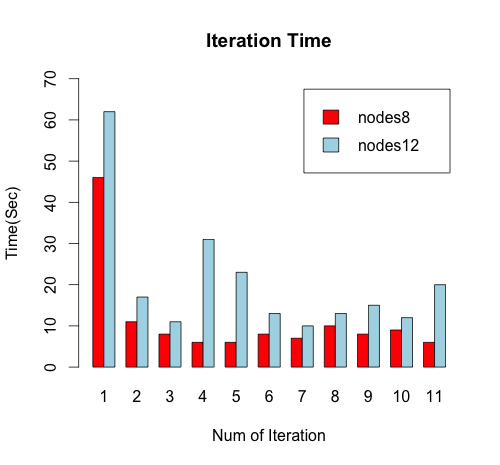
\includegraphics[width=90mm]{images/in-mem.png}
        \caption{In-Memory RDD for iterative algorithms}
        \label{fig:in-memory}
    \end{figure}

The main technical insight behind Spark is the Resilient Distributed Dataset,
which resides in memory and stays in memory over the iterations, while Hadoop
incurs I/O penalties because it materializes intermediate data (like the map
output) on disk before the data is shuffled. As such, we ran a test to see
how total wall clock time changed from one run to the next.

We tested a simple PageRank implementation on a dataset with 1.4 million pages
and 50 million links in total on 8 nodes and 12 nodes, ensuring that there
is enough heap space for all of the data to fit into memory. We set
the number of iterations to be 11. During the first iteration, the program
needs to load the data from the disk and then process the data. As shown in
Figure \ref{fig:in-memory} for both the 8-node cluster and 12-node cluster, the
time spent on the first iteration is much higher than all the latter
iterations. Note that the time for 12-node cluster is always
higher than 8-node cluster because the dataset is small and the performance
gain from distributing the work is less than the communication overhead
incurred with more nodes. In sum, in-memory dataset does improve the
performance for iterative algorithms.

Spark often stores the whole dataset in memory in order to avoid disk I/O.
However, when there is not sufficient memory to do this, disk I/O is
unavoidable.  As such, Spark has an algorithm to swap the least-used
data to disk and keeps the most-used in memory. This test is to find how
the performance degrades as we restrict the amount of heap space.


\begin{figure}[H]
        \centering
        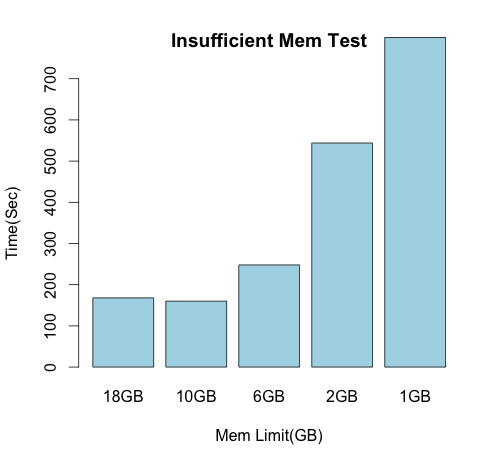
\includegraphics[width=90mm]{images/insufficient_memory.png}
        \caption{Insufficient memory test}
        \label{fig:insuff-mem}
    \end{figure}

For comparison, we tested a Bagel implementation of PageRank on a dataset with
64,000 pages and 30 million links in total on four nodes in Janus. As we limit
the memory size from 1GB to 18GB in each node, the time is recorded. As shown
in the Figure \ref{fig:insuff-mem}, the time stays stable when the memory limit
is over 6GB since the program won’t use disk for RDD data storage. Once the
memory limit is less than the memory required, the performance drops until it
fails on one-node cluster, where the Java heap allocation is exceeded. Despite
the performance degradation, it's quite linear. Besides, the dataset size is
4.2GB and it consumes around 8.8GB memory per node, which is 35GB of memory in
total. One of the reasons is that RDDs are immutable and every time a RDD is
transformed, a new RDD is created, thus taking up lots of memory. The other
reason is that Spark replicates the RDD on the go for loss of data.

\begin{figure}[H]
        \centering
        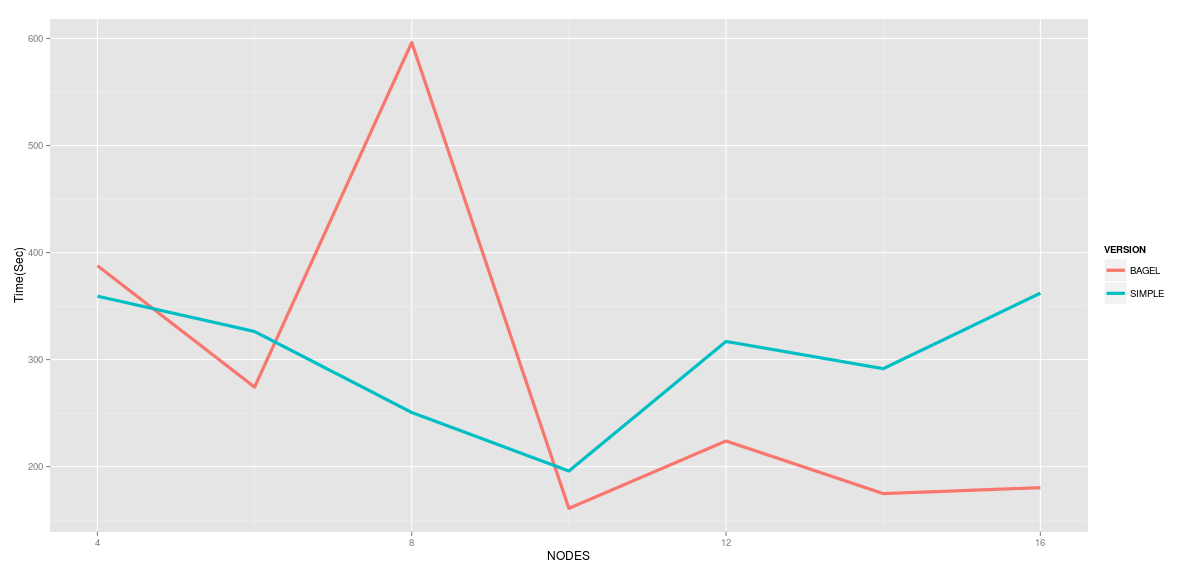
\includegraphics[width=90mm]{images/bagelsimple.png}
        \caption{Bagel VS. Simple PageRank}
        \label{fig:bagelsimple}
    \end{figure}

In order to measure the relative performance of the Bagel and simple
implementations, we ran both versions of PageRank on
number of nodes from 4 to 16 with increment 2 and a dataset with 64,000 pages and
30 million links in total with sufficient memory. In Figure
\ref{fig:bagelsimple} regardless of time, we can see that bagel version
outperforms simple version a little bit. The main reason is that for a smaller
dataset, the overhead of managing vertices, edges and messages are so huge that
the benefits of asynchronous background messages that Spark might offer is not
that obvious. We couldn’t test on big dataset because of the aforementioned
technical failure. However, it's worth noting that programming is easier with
general concepts of vertices, edges and messages to represent the graph.

\begin{figure}[H]
        \centering
        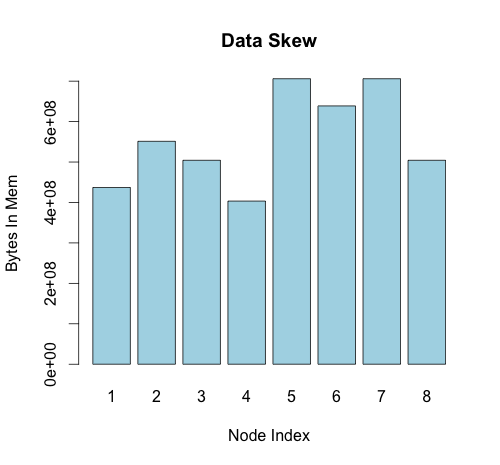
\includegraphics[width=90mm]{images/skew.png}
        \caption{Data Skew Test}
        \label{fig:dataskew}
    \end{figure}

Finally, we will focus on the potential data skew problem, which exists in systems
like Hadoop. Since with data skew, a single straggler could slow down the whole
program considerably.

We ran our Bagel version of PageRank on four nodes and on dataset of 30 million
links. As shown in Figure \ref{fig:dataskew}, the memory used is quite balanced
across the nodes. We checked the data size read from the disk and found that
all the nodes are reading the exact same amount of data from the disk. So the
little imbalance came from the RDDs created later, which is partitioned by a
certain key.

% pagerank test 1
% pagerank test 2
% ...

\section{Discussion}
The results collected from the initial grep test over the 20 GB file gave us
some insight on how well such a problem scales in the Spark system. Given a
text file of 20 GB, it appears that employing 3 nodes provides a good balance
between speedup and efficiency. We also saw how the number of workers per node
effects the overall runtime. While 1 to 3 workers yield relatively similar
results, it seems that using 2 to 3 nodes may give a slight performance
increase. This test would need to be run several more times to achieve more
more conclusive runtime averages. It would also be beneficial to increase the
input file size and node counts, to see if the observed trend continues as the
problem is scaled up.

In the grep test over the 100 GB file, surprisingly we observed practically no
change in runtime performance. Perhaps the Karp-Flatt metric results seen in the
previous test gives us some insight as to why this is the case. We suspect the
long load times on this larger file greatly outweigh any speedup achieved
through running grep on multiple workers. Given that, we also suspect that
Spark could be reading this file serially from the lustre file system. The
lack of Spark logging and profiling tools makes it difficult to determine
exactly how long each stage is taking. Further investigation would be needed
to determine a possible solution or workaround.

To sum up, Spark, with its in memory data store, performs great on iterative
algorithms and degrade linearly with insufficient memory. Using a partitioner,
the dataset is uniformly distributed across the nodes to avoidance of possible
stragglers. For the scalability test, the time increase with the number of nodes
is due to the communication overhead for the small dataset. We believe that
solving the akka error would enable the program to run on larger datasets, and
show great scalability nodes counts of 10 and under. 

The biggest problem we had throughout these tests was the akka failure. This
occurs when we ran large dataset on a small number of nodes. This prevented us
from increasing the ratio of computing to communication for scalability test.
Secondly, due to the time limit for a cluster of allocated nodes on JANUS, we
have to stop in the middle of testing and reallocate nodes. This often
reflected in inconsistent results. It might be that the nodes we reallocate
have different network topology with network congestion. Finally, although we
ran three trials for each test, we saw a significant difference in time,
despite running with the same exact configuration. To help address this issue,
we simply discarded any result that appeared to be an outlier as compared to
the other two results.

% pagerank test 1
% pagerank test 2
% ...

% other problems exhibited
    % easy to install, hard to configure/profile/understand results
    % sporadic runtimes 

% workers and master communication over spark protocol

\section{Conclusion}
We found that, while Spark offers an appealing abstraction layer for
data-parallel programming, achieving reasonable scalability even on trivial
problems is still very difficult. Any abstraction for parallelism would
seemingly run into this problem: when speedups are not as expected, it is often
much harder to track down the source of the problem.  The lack of adequate
profiling tools made the lackluster results of our experiments all the more
puzzling. With more time, we could probably use the Spark logs to better
understand where our serial bottlenecks are and increase efficiency. It may
very well still be worth exploring how Spark could be used on JANUS, but it may
require rethinking how we are using the network and filesystems for this task.

\bibliography{paper}
\bibliographystyle{plain}

\end{document}
